\documentclass[fontsize=12pt,paper=a4,twoside]{scrartcl}

\usepackage{graphicx}
\usepackage{listings}
\usepackage[ngerman]{babel}

% SWP-Präambel
% C 2003-2017 Sebastian Offermann, Rainer Koschke, Karsten Hölscher
% In Zeilen 40 und 41 sind jeweils die aktuellen Daten einzutragen

\usepackage[utf8]{inputenc}     % Kodierung der Tex-Datei
\usepackage[T1]{fontenc}        % Korrekte Ausgabe von Sonderzeichen (Umlaute)
\usepackage[ngerman]{babel}     % Deutsche Einstellungen [ab \begin{document}]

\usepackage{bibgerm}            % Bibliographie
\usepackage{fancyhdr}           % obere Seitenränder gestalten
\usepackage{float}              % Floats Objekte mit [H] festsetzen
\usepackage{graphicx}           % Graphiken als jpg, png etc. einbinden
\usepackage{moreverb}           % zusätzliche verbatim-Umgebungen
\usepackage{pdflscape}          % PDF-Support für landscape
\usepackage[final]{pdfpages}    % Externe PDFs einbinden
\usepackage{stmaryrd}           % zusätzliche Symbole
\usepackage{supertabular}       % Tabellen über Seitenränder hinaus
\usepackage{tabularx}           % Tabellen mit vorgegebener Breite
\usepackage{url}                % setzt URLs schön mit \url{http://bla.laber.com/~mypage}

%%% Die Reihenfolge der folgenden Pakete muss beibehalten werden:
%%% varioref, hyperref, cleveref, bookmark
% Verweise innerhalb des Dokuments schick mit " ... auf Seite ... "
% automatisch versehen. Dazu \vref{labelname} benutzen
\usepackage[ngerman]{varioref}  % [vor hyperref für korrekte Verweise]
\usepackage[colorlinks=true, pdfstartview=FitV, linkcolor=blue,
            citecolor=blue, urlcolor=blue, hyperfigures=true,
            pdftex=true]{hyperref} % [vor bookmark wegen der Optionen]
\usepackage[ngerman]{cleveref}
\usepackage{bookmark}

\hyphenation{Arbeits-paket}     % Trennungsregeln

%%% Definitionen
\newcommand{\grad}{\ensuremath{^{\circ}} }
\renewcommand{\strut}{\vrule width 0pt height5mm depth2mm}
\newcommand{\gq}[1]{\glqq{}#1\grqq{}}

%%% Semesterkonstanten
\newboolean{langversion} %Deklaration
\setboolean{langversion}{true} %Zuweisung ist 'false' für Blockkurs
\newcommand{\jahr}[1]{2020} %2017/2018

% erstes Argument: SWP-2, zweites SWP-1
\newcommand{\highlight}[1]{\textcolor{blue}{\textbf{#1}}}
\newcommand{\variante}[2]{\ifthenelse{\boolean{langversion}}{#1}{#2}}
\newcommand{\nurlangversion}[0]%
    {\variante{\highlight{}}%Muss in SWP-2 ausgefüllt werden}}%
              {\highlight{Entfällt in SWP-1}}}
\newcommand{\swp}[0]{Software-Projekt \variante{2}{1}}
\newcommand{\semester}[0]{SoSe \jahr}

%%% Formatierungsanpassungen
% Damit Latex nicht zu lange Zeilen produziert:
\sloppy
%Uneinheitlicher unterer Seitenrand:
%\raggedbottom

% Kein Erstzeileneinzug beim Absatzanfang
% Sieht aber nur gut aus, wenn man zwischen Absätzen viel Platz einbaut
\setlength{\parindent}{0ex}

% Abstand zwischen zwei Absätzen
\setlength{\parskip}{1ex}

% Seitenränder für Korrekturen verändern
\addtolength{\evensidemargin}{-1cm}
\addtolength{\oddsidemargin}{1cm}

\bibliographystyle{gerapali}

% 1. Parameter: Euer/Eure TutorIn, z. B. {Kim Harrison}
% 2. Parameter: Abgabedatum, z. B. {05. April 2063}
% 3. Parameter: Versionsnummer, z. B. {1.1}
% 4.-9. Parameter: jeweils Name und (Uni-)Email-Adresse jedes 
%                 Gruppenmitglieds; mit einem & getrennt, z. B.
% {Robin Cowl & roco@tzi.de}
% Besteht die Gruppe aus weniger als 6 Personen, so werden die 
% übrigen Parameter leer gelassen: {}
\newcommand \swpdocument[9] {
% Lustige Header auf den Seiten
  \pagestyle{fancy}
  \setlength{\headheight}{70.55003pt}
  \fancyhead{}
  \fancyhead[LO,RE]{\swp{}\\%
                    \semester{}\\%
                    \documentTitle}
  \fancyhead[LE,RO]{Seite \thepage\\%
                    \slshape \leftmark\\%
                    \slshape \rightmark}

% Lustige Header nur auf dieser Seite (Titelseite)
  \thispagestyle{fancy}
  \fancyhead[LO,RE]{ }
  \fancyhead[LE,RO]{Universität Bremen\\%
                    FB 3 -- Informatik\\%
                    Dr. Karsten Hölscher\\%
                    TutorIn: #1}
  \fancyfoot[C]{}

% Start Titelseite
  \vspace{3cm}
  \begin{minipage}[H]{\textwidth}
    \begin{center}
      \bfseries \Large \swp{} -- \semester{}\\
      \smallskip
      \small VAK 03-BA-901.02\\
      \vspace{3cm}
    \end{center}
  \end{minipage}
  \begin{minipage}[H]{\textwidth}
    \begin{center}
      \vspace{1cm}
      \bfseries \Large \documentTitle\\
      \vfill
    \end{center}
  \end{minipage}
  \vfill
  \begin{minipage}[H]{\textwidth}
    \begin{center}
      \sffamily
      \begin{tabular}{lr}
        #4 \\
        #5 \\
        #6 \\
        #7 \\
        #8 \\
        #9 \\
      \end{tabular}
      \\[22mm]
      \itshape Abgabe: #2 --- Version #3 \\ ~
    \end{center}
  \end{minipage}
% Ende Titelseite

% Start Inhaltsverzeichnis
\newpage
  \thispagestyle{fancy}
  \fancyhead{}
  \fancyhead[LO,RE]{\swp{}\\%
                    \semester{}\\%
                    \documentTitle}
  \fancyhead[LE,RO]{Seite \thepage\\%
                    \slshape \leftmark\\~}
  \fancyfoot{}
  \renewcommand{\headrulewidth}{0.4pt}
  \tableofcontents
% Ende Inhaltsverzeichnis

% Header für alle weiteren Seiten
\newpage
  \fancyhead[LE,RO]{Seite \thepage\\%
                    \slshape \leftmark\\%
                    \slshape \rightmark}

}



\begin{document}

\tableofcontents

\newpage

% ==================== Installation ====================
%\setcounter{chapter}{1}

\section{Installation}

Um das Programm zu installieren, benötigen sie zunächst sowohl eine valide JDK installation, als auch eine Gradle installation. Wenn sie eine der beiden nicht haben, verfolgen sie bitte folgenden zwei Installationsanleitungen. Sollten sie sowohl eine JDK als auch eine Gradle Installation schon haben, so können sie bei Punkt 0.0.3 weiterlesen.

% ==================== JDK INSTALLATION ====================
\subsection{JDK Installation}

Sie benötigen zunächst eine valide JDK Installation. JDK steht für Java Development Kit und wird verwendet um Java Programme zu entwickeln.
Bei unserem Programm können sie eine beliebige JDK mit einer Version von 8+ herunterladen. Wir werden die Vorgehensweise einer Installation von JDK  8 als Beispiel durchführen.

% ==================== WINDOWS ====================
\subsubsection{Windows JDK Installation}

Navigieren sie bitte auf die Webseite https://www.ninite.com . Ninite ist eine Webseite mit welcher man mehrere Programme gleichzeitig automatisiert herunterladen kann. Dort werden sie unter ''Developer Tools'' eine JDK Version mit dem Namen ''JDK (AdoptOpenJDK) x64 8'' sehen. Kreuzen sie die box daneben mit einem Mausclick an. Scrollen sie nun ganz herunter und clicken sie auf den Knopt ''Get Your Ninite''. Führen sie die heruntergeladene Datei aus, welche dann automatisch JDK 8 installieren wird.

\begin{figure}[h!]
\centering
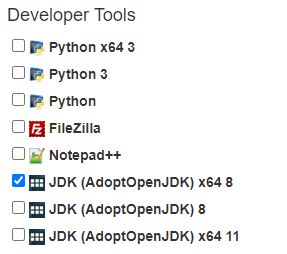
\includegraphics[width=0.5\linewidth]{Windows.JPG}
\end{figure}

Um zu verifizieren das JDK korrekt installiert wurde, öffnen sie ein CMD oder Powershell Fenster, entweder durch ihre Apps oder mit Strg + R, tippen sie dann CMD oder Powershell und drücken sie Enter. Geben sie im geöffneten Fenster das Kommando Javac ein und drücken sie Enter. Sollte nichts passieren, und sie einen Fehler bekommen, so wurde das JDK nicht korrekt installiert und sie müssen das folgende Subkapitel auch noch durchgehen. Wird das Kommando wie im Bild korrekt ausgeführt, so können sie beim Kapitel ''Gradle Installation'' weiterlesen. 

\begin{figure}[h!]
\centering
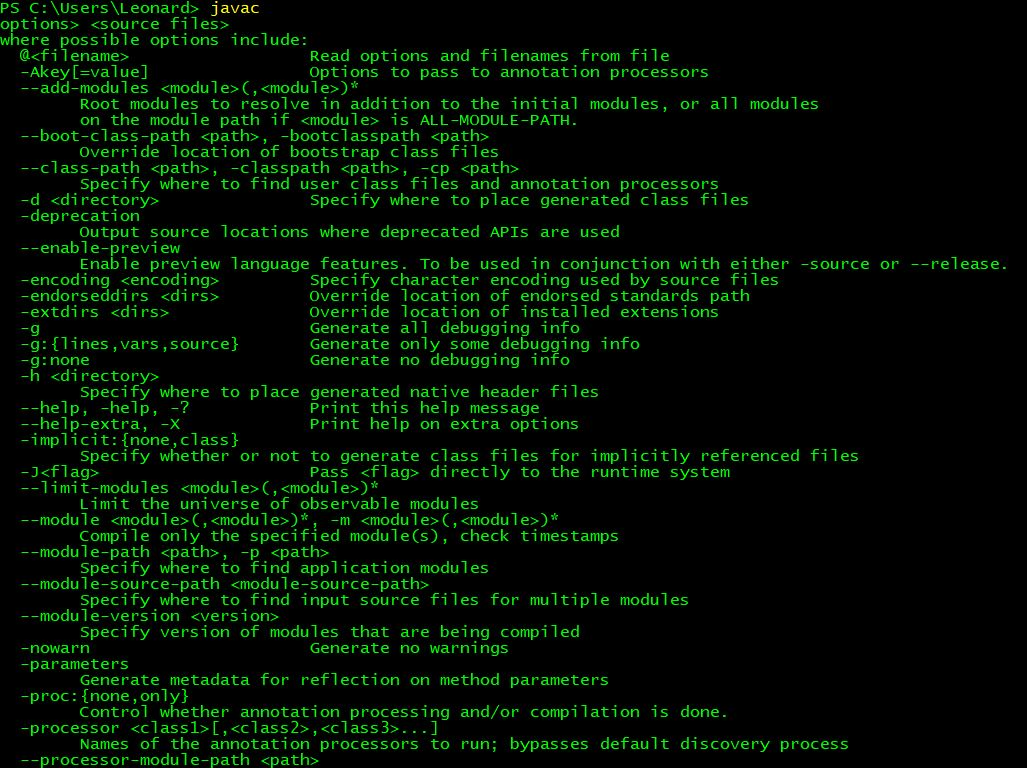
\includegraphics[width=\linewidth]{JavacWindows.JPG}
\end{figure}


\newpage
\paragraph{PATH und JAVA\textunderscore HOME}

Sollte das Kommando im letzten Schritt ein Fehler angezeigt haben, so ist JDK nicht korrekt konfiguriert. Um dieses zu ändern, navigieren sie bitte zu dem Installationspfad ihrer Jdk, welcher einen Namen wie ''C:/Program Files/Java/jdk-version haben wird''. In diesem Ordner werden sie einen weiteren Ordner ''bin'' finden und erst einmal öffnen. Kopieren sie nun den Pfad dieses Ordners (z.B. ''C:/Program Files/Java/jdk-12.0.2/bin'' für JDK 12.0.2) und öffnen sie unter Windows XP/7 My PC, oder unter Windows 8+/10 This PC. Clicken sie die rechte Maustaste und wählen sie ''Properties'' aus.
\begin{figure}[h!]
\centering
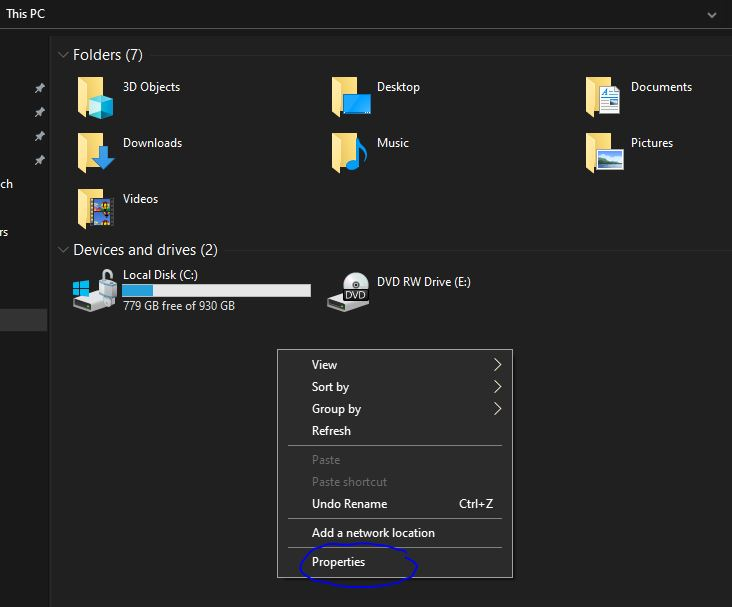
\includegraphics[width=0.7\linewidth]{Properties.JPG}
\end{figure}

In dem geöffneten Fenster auf der linken Seite werden sie einen Knopf ''Advanced System Settings'' sehen, welchen sie nun anclicken.
\begin{figure}[h!]
\centering
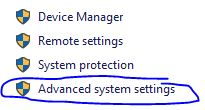
\includegraphics[width=0.5\linewidth]{AdvancedSystemSettings.JPG}
\end{figure}

\newpage
In dem nun geöffneten Fenster, ganz unten Rechts, clicken sie auf den Knopf ''Environment Variables''.
\begin{figure}[h!]
\centering
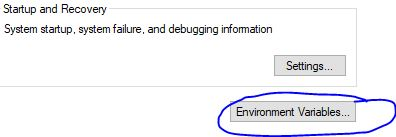
\includegraphics[width=0.5\linewidth]{EnvironmentVariables.JPG}
\end{figure}

Hier sind alle Variablen von Programmen die Windows durch die Konsole erkennt vorhanden. Wr müssen nun unsere JDK Installation dazufügen. Um dieses zu tun, clicken sie bei den ''System Variables'' auf den ''New...'' Knopf und geben der Variable den Namen ''JAVA\textunderscore HOME'', beachten sie das der Name korrekt und groß geschrieben ist, und als Pfad geben sie den kopierten Pfad ohne die ''/bin'' endung an, also z.B. '''C:/Program Files/Java/jdk-12.0.2'' und clicken sie dann auf Ok.
\begin{figure}[h!]
\centering
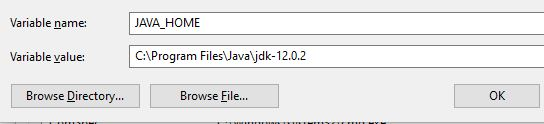
\includegraphics[width=\linewidth]{JAVA_HOME.JPG}
\end{figure} 

\textbf{(*)}
Jetzt müssen sie nur noch ihre System PATH Variable bearbeiten um Java als System Variable einzufügen. Um dieses zu tun, scrollen sie unter ''System Variables'' runter bis sie eine Variable mit dem Namen ''Path'' sehen, und dann diese doppelclicken. In dem jetzt angezeigtem Fenster sind sämtliche Programme die von Windows als System Variablen erkannt werden drin. Clicken sie rechts auf ''New'' und fügen sie den gesamten kopierten Pfad ein und drücken sie Enter. Sie können nun alle Fenster schließen. 
\begin{figure}[h!]
\centering
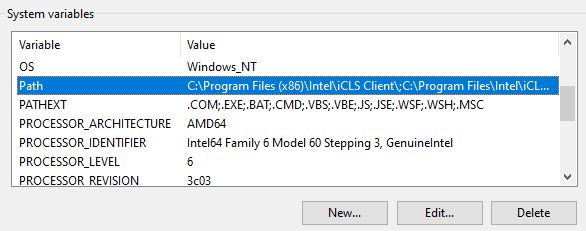
\includegraphics[width=\linewidth]{SystemVariables.JPG}
\end{figure} 

\textbf{(*) Für die Installation auf anderen Betriebssystemen, lesen sie bitte die Dokumentation auf der JDK Oracle Webseite.}

% ==================== LINUX ====================
% TODO ADD LINUX AND MACOS

% ==================== GRADLE INSTALLATION ====================
\subsection{Gradle Installation}

Nun werden wir Gradle installieren. Gradle is ein ein Tool mit welchem man Java Applikationen bauen kann.

% ==================== WINDOWS ======================
\subsubsection{Windows Gradle Installation}

Navigieren sie auf die Webseite https://gradle.org/install/ und scrollen sie runter zu ''Installing manually''. Clicken sie dort auf ''Binary-only'' welches Gradle herunterladen sollte.
\begin{figure}[h!]
\centering
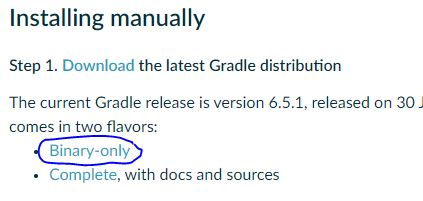
\includegraphics[width=0.5\linewidth]{GradleDownload.JPG}
\end{figure} 

Extrahieren sie die heruntergeladene ZIP datei und kopieren sie den Pfad der bin datei in der Gradle datei, z.B. ''PFAD/gradle-6.4.1/bin'' und erstellen für diesen einen neuen Eintrag in der System Path Variable, siehe (*) bei der JDK Installation. Sie sollten nun die Möglichkeit haben in einem CMD oder Powershell fenster das Kommando ''gradle -version'' ausführen zu können.

\textbf{(*) Für die Installation auf anderen Betriebssystemen, lesen sie bitte die Dokumentation auf der Gradle Webseite.}

% ==================== JRE ====================

\subsection{Java Installation (JRE)}

Um das Programm ausführen zu können, werden sie eine normale Java Installation benötigen. Der Unterschied zwischen der JRE (Java Runtime Environment) und der JDK, ist das die JDK zur Entwicklung von Java Programmen gedacht ist, die JRE aber zur Ausführung dieser Programme benutzt wird. Um die neuste JRE zu installieren, navigieren sie einfach in ihrem Browser auf die Webseite https://www.java.com/download und laden sie sich Java herunter.(Clicken sie einfach immer auf weiter in der Installation)

(*) Wenn sie möchten dass das Programm schneller läuft, so können sie dem mehr Arbeitsspeicher zur Verfügung stellen. Hierbei ist die 32 bit JRE allerdings auf 2GB beschränkt, also könnten sie sich gleich eine 64 bit JRE herunterladen.

% ==================== Application Installation ==================== 

\subsection{Installation der Software}

Nachdem sie nun alle obigen Programme installiert haben, können sie nun endlich die Applikation selbst installieren. Navigieren sie hierzu bitte in den Ordner der Software (galaxytrucker in der Regel), öffnen sie eine Konsole ihrer Wahl und führen sie das Kommando ''gradle clean desktop:dist'' aus. Sollte ihre Gradle Version hiermit Probleme haben, so können sie auch den Projekt begleitendem gradlew File benutzen, indem sie stattdessen das Kommando ''.\textbackslash gradlew clean desktop:dist'' ausführen. (Unter Windows funktioniert letzteres nur in Powershell und nicht in CMD)  
\begin{figure}[h!]
\centering

\includegraphics[width=0.5\linewidth]{command.JPG}
\end{figure} 
\textbf{Der Gradle Build wird zwar ganz viele Warnungen geben, dieses liegt allerdings da dran das Gradle nicht versteht wozu die @NonNull tags gedacht sind, also ignorieren sie diese.}

Nachdem sie die Nachricht ''BUILD SUCCESSFUL'' bekommen, können sie die Programmdatei im Unterordner ''desktop$\rightarrow$build$\rightarrow$libs'' finden. Es wird eine Datei vom Format JAR sein und wahrscheinlich den Namen ''desktop-1.0.jar'' haben.

\begin{figure}[h!]
\centering
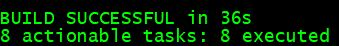
\includegraphics[width=0.5\linewidth]{gradle_build.JPG}
\end{figure} 

\begin{figure}[h!]
\centering
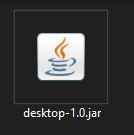
\includegraphics[width=0.5\linewidth]{application.JPG}
\end{figure} 

% ==================== Running Application ==================== 

\subsection{Programmausführung}

Um das Programm nun auszuführen, können sie entweder die JAR durch doppelklick direkt ausführen, oder, wenn sie dem Programm mehr Arbeitsspeicher zur Verfügung stellen wollen (damit es schneller läuft), dieses mit dem Kommando ''java -Xms1G -Xmx4G -jar .\textbackslash desktop-1.0,jar'' starten. Letzteres wird dem Programm mindestens 1 GB Arbeitsspeicher  (Xms steht für Minimum) und bis zu maximal 4 GB Arbeitsspeicher yur Verfügung stellen (Xmx steht für Maximum).

\begin{figure}[h!]
\centering
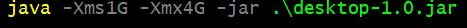
\includegraphics[width=0.8\linewidth]{run_application.JPG}
\end{figure} 

% ==================== The Application ==================== 

\section{Menüs}

\subsection{Hauptmenü}

\subsubsection{Multiplayer}

\subsection{Optionen}

%%%%%%%%%%%%%%%%%%%%%%%%%%%%%%%%%%%%

\section{Das Spiel}

%allgemeine Erklärung was alles ist

\subsection{Schiff Interface}

%nähere Erklärungen zu allen Punkten

\subsubsection{Energiemanagement}

\subsubsection{Schiffinformationen}

\subsubsection{Waffen}


\subsection{Inventar (Ship)}


\subsection{Karte (Jump)}

Das Kartenfenster wird im Spiel mit einem Klick auf den Jump-Button geöffnet. 
\begin{figure}[h!]
\centering
\includegraphics[width=1\linewidth]{DasSpiel/Karte/karteübersicht.png}
\end{figure} 

-----HIER ZAHLEN EINFÜGEN, Textur der Map verändern-----

Das kleine Schiff (1) Zeigt dem Spieler immer an, auf welchem Planeten er sich gerade Befindet. Hier in dem Beispiel befindet der Spieler sich auf dem Startplaneten. 

Die eingekreisten Punkte (2) sind Planeten, welche das während des Spiels existieren. Bei jedem neu erstellten Spiel wird eine zufällig generierte, einzigartige Karte mit Events auf jedem Planeten erstellt erstellt. 

Das rot hinterlegte Raumschiff (3) ist der Endboss des Spiels. 

\subsubsection{Planeten}

\paragraph{Startplanet: }
Der Startplanet existiert auf jeder Map nur einmal. Hier gibt es kein Event. Dieser Planet dient dazu, dass man in Ruhe am Anfang des Spiels sich seine Ausrüstung erstmal anschauen kann. 

\paragraph{Normale Planeten: }
Die normalen Planeten sind eine Zufällig generierte Anzahl an Planeten, auf denen Zufällig eins aus 6 Events auftritt:

\subparagraph{Kein Event} Hier Kann es zu einem Zufälligen Geschenk kommen, welches dem Inventar hinzugefügt wird. 
\subparagraph{Nebel} Hier kann es zufällige Geschenke geben, die dem Spieler zugeschrieben werden.
\subparagraph{Meteoritenfeld} Hier kann es zu Schäden am Schiff kommen, welche dem Spieler mit Verlust zufälliger Resourcen kenntlich gemacht wird. Es ist außerdem möglich, Zufällige Resourcen zu finden (Geschenk).
\subparagraph{Gegnerisches Schiff} Hier kann man ein zufälliges Geschenk erhalten. Hier wird ein gegnerisches Schiff angezeigt, welches im folgenden Bekämpft werden muss (Siehe Kampf). Die normalen Gegner haben immer die gleichen Stats und Waffen, welche der Grundausstattung der Schiffe entspricht, aus denen der Spieler auch auswählen kann. Beim Gewinnen bekommt der Spieler eine zufällige Auswahl an Sachen geschenkt. 
\subparagraph{Gegnerisches Schiff (Miniboss)} Das Miniboss Planetevent gleicht dem normalen Gegnerischen Schiff Event, nur dass der Gegner an die Stats des Spielers angepasst wird. Er bekommt ähnlich gute Waffen und ein ähnlich hohes leben, sodass das Besiegen schwerer ist. Beim Gewinnen bekommt der Spieler eine zufällige Auswahl an Sachen geschenkt. 
\subparagraph{Shop} Beim Shop ist es dem Spieler möglich, Ausrüstung zu kaufen oder zu verkaufen. (Siehe Kapitel Shop)

\subsubsection{Symbole}


\subsection{Shop}


\subsection{Kämpfe}

\subsubsection{Erklärung}

\subsubsection{Mögliche Taktiken}























\end{document}